\documentclass{article}

\usepackage[
margin=0in,
paperwidth=12.705in,  % 6.125 + 0.455 + 6.125  (WHITE, 202 pages)
paperheight=9.25in
]{geometry}

\usepackage{graphicx}
\usepackage{tikz}
\usetikzlibrary{calc}
\usepackage{xcolor}
\pagestyle{empty}

% Dimensions
\newlength{\panel}
\setlength{\panel}{6.125in}    % each side including bleed

\newlength{\spine}
\setlength{\spine}{0.455in}    % spine width (white paper, 202 pages)

\newlength{\coverheight}
\setlength{\coverheight}{9.25in}

% Colors
\definecolor{coverblue}{HTML}{1E4A66}  % spine text color
%\definecolor{spinebg}{HTML}{D9CFC1} % neutral gray-beige, subtle contrast
%\definecolor{spinebg}{HTML}{CFC0A9} % darker cream, stronger contrast
%\definecolor{spinebg}{HTML}{F0E8D6} % subtle spine background
\definecolor{spinebg}{HTML}{E6D8B9} % warm beige, slightly stronger

\begin{document}
	
	\begin{tikzpicture}[remember picture,overlay]
		
		% Page reference
		\coordinate (SW) at (current page.south west);
		
		% --- Back cover on the left ---
		\node[anchor=south west, inner sep=0pt] at (SW)
		{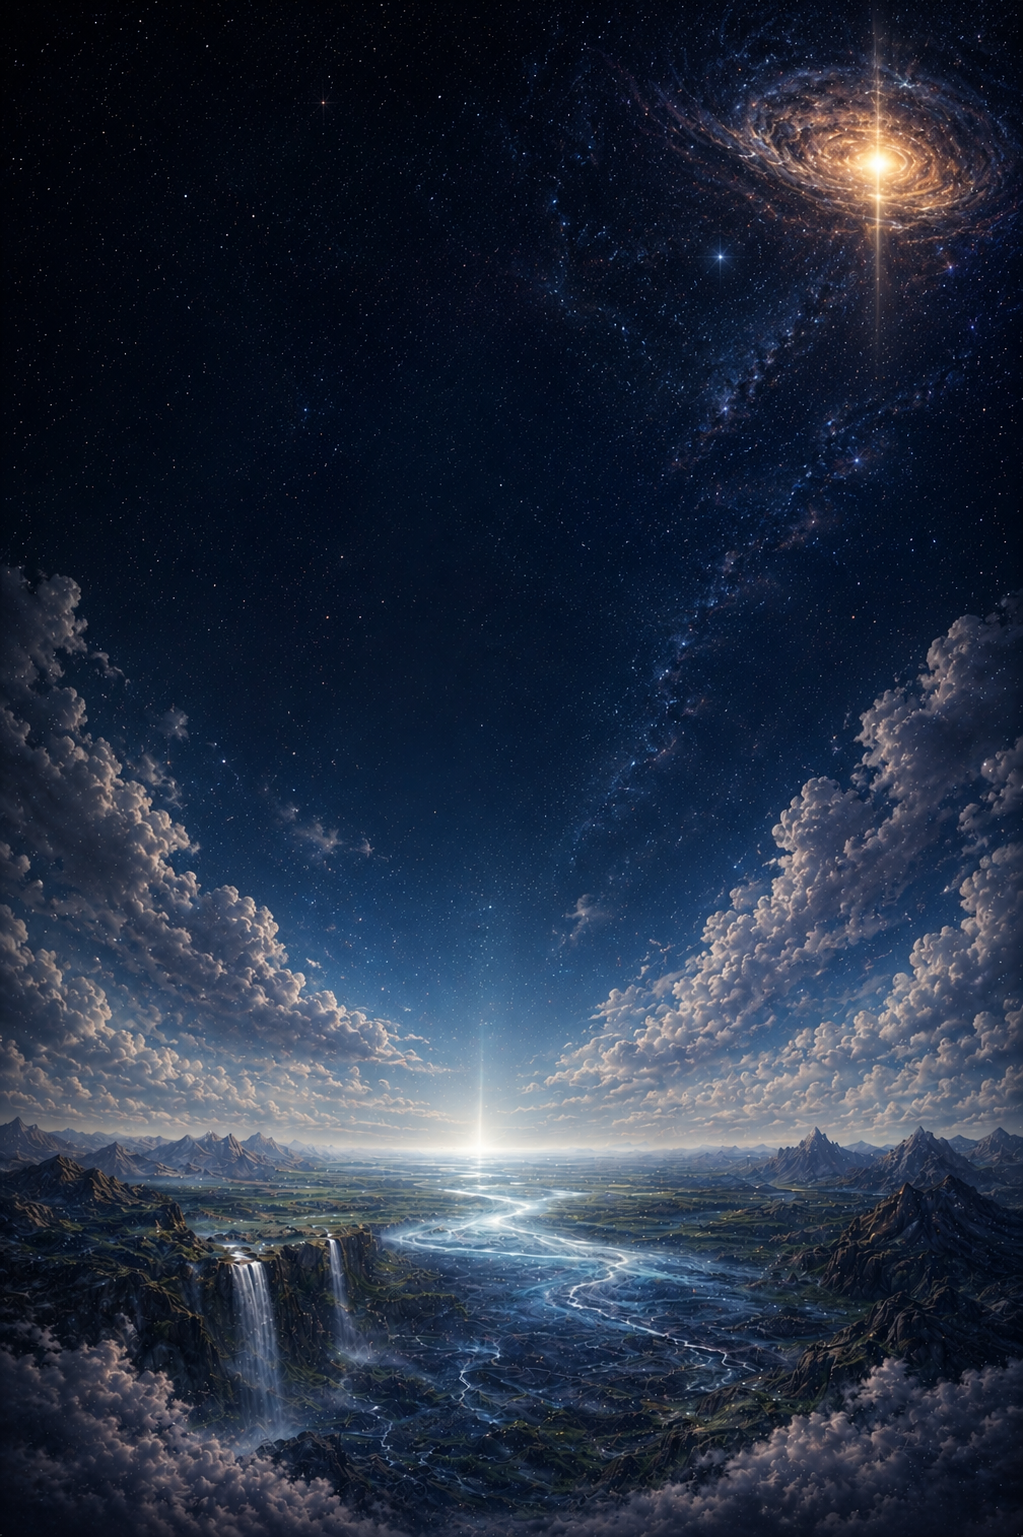
\includegraphics[width=\panel,height=\coverheight]{rueckseite.pdf}};
		
		% --- Spine in the center ---
		\fill[spinebg] 
		($(SW)+(\panel,0)$) 
		rectangle 
		++(\spine,\coverheight);
		
		% --- Front cover on the right ---
		\node[anchor=south west, inner sep=0pt]
		at ($(SW)+(\panel+\spine,0)$)
		{\includegraphics[width=\panel,height=\coverheight]{vorderseite.pdf}};
		
		% --- Spine text, rotated 90 degrees and centered ---
		\node[rotate=90, align=center, text=coverblue]
		at ($(SW)+(\panel+0.5*\spine,0.5*\coverheight)$)
		{
			\bfseries\normalsize
			Christian Weilharter
			\hspace*{0.8cm}
			The Structure of the World
		};
		
		% -------------------------------------------------
		% Kontrolllinien: später auskommentieren
		% -------------------------------------------------
		
		% Linke Rückenkante
		%\draw[red, line width=0.3pt] 
	%	($(SW)+(\panel,0)$) -- ($(SW)+(\panel,\coverheight)$);
		
		% Rechte Rückenkante
		%\draw[red, line width=0.3pt] 
		%($(SW)+(\panel+\spine,0)$) -- ($(SW)+(\panel+\spine,\coverheight)$);
		
		% Rückenmitte
		%\draw[blue, line width=0.3pt] 
		%($(SW)+(\panel+0.5*\spine,0)$) -- ($(SW)+(\panel+0.5*\spine,\coverheight)$);
		
	\end{tikzpicture}
	
\end{document}